%%
%% Author: Fabian Klopfer (fabian.klopfer@ieee.org) 
%%

% Preamble
\documentclass[a4paper]{article}

% Packages
\usepackage[utf8]{inputenc}
\usepackage[T1]{fontenc}
\usepackage{enumerate}
\usepackage{fancyhdr}
\usepackage{amssymb}
\usepackage{amsmath}
\usepackage{amsfonts}
\usepackage{a4wide}
\usepackage{graphicx}
\usepackage{wrapfig}
\usepackage{tikz}
\usetikzlibrary{automata,positioning}
\usepackage{listings}
\usepackage{colortbl}
\usepackage{tabularx}
\usepackage{hyperref}
\usepackage{multicol}
\usepackage{float}

\setlength{\headheight}{24pt}

\pagestyle{fancy}
\lhead{Fabian Klopfer (956507)}
\rhead{Probabilistic Modelling\\Assignment 2}

	\newcommand{\pmat}{\begin{pmatrix}	
	0 			& \frac{3}{4} & 0 			& \frac{1}{4} \\[3pt]
	\frac{1}{3} & 0			  & \frac{1}{6} & \frac{1}{2} \\[3pt]
	0			& 0			  & 1 			& 0			  \\[3pt]
	0			& \frac{1}{4} & \frac{1}{2}	& \frac{1}{4} \\[3pt]
	\end{pmatrix} }
	
	\newcommand{\pppmat}{\begin{pmatrix}	
	0.02083333 			& 0.296875 & 0.47916667 			& 0.203125 \\
	0.125 & 0.05208333			  & 0.58333333 & 0.23958333 \\
	0			& 0			  & 1 			& 0			  \\
	0.02083333			& 0.109375 & 0.77083333	& 0.09895833 \\
	\end{pmatrix} }

% Document
\begin{document}
	
	\section*{Exercise 1: Probabilities in DTMCs}\label{sec:exercise1}
	Let the transition matrix $P$: 
	\[  P = \pmat \]
   \begin{enumerate}[a.]
       \item Compute $P^3(s_0,s_3)$ \\
       Using the Chapman-Kolmogorov equation:
           \[ p_{s_0,s_3} (3) = \sum_{s'} p_{s_0, s'}(l) p_{s', s_3}(3 - l) = \sum_{s'} P(s_0, s') p_{s', s_3}(2)  =  \sum_{s'} P(s_0, s') (\sum_{s''} P(s', s'') P(s'', s_3))\]
           \[  \Leftrightarrow  \sum_{s'} P(s_0, s') (P(s',s_1) P(s_1, s_3) + P(s', s_0) P (s_0, s_3) + P(s', s_3)P(s_3, s_3))  \]
            \[  \Leftrightarrow  P(s_0, s_3)P(s_3, s_1) P(s_1, s_3) + P(s_0, s_1)  P(s_1, s_0) P(s_0, s_3)  +  P(s_0, s_3)P(s_3, s_3)P(s_3, s_3) \]
            \[ + P(s_0, s_1) P(s_1, s_3) P(s_3, s_3) \]
             \[  \Leftrightarrow  \frac{1}{4} \cdot \frac{1}{4} \cdot \frac{1}{2} + \frac{3}{4} \cdot \frac{1}{3} \cdot \frac{1}{4}  +  \frac{1}{4} \cdot \frac{1}{4} \cdot \frac{1}{4} +  \frac{3}{4} \cdot \frac{1}{2} \cdot \frac{1}{4} \]
             \[ \Leftrightarrow \frac{1}{32} + \frac{3}{48} + \frac{1}{64} + \frac{3}{32} = \frac{2}{64} + \frac{4}{64} + \frac{1}{64} + \frac{6}{64} \]
             \[ \Leftrightarrow \frac{13}{64} = 0.203125\]
             \[ \Leftrightarrow \pppmat \huge\vert_{(s_0,s_3)} \]
             \[ \Leftrightarrow \pmat^3 \huge\vert_{(s_0,s_3)} = P^3(s_0, s_3) \]
             
        \item Compute the probability of being in state s3 after exactly 3 steps assuming a uniform initial  distribution (over all states).
            \[ \Theta_3^{\mathcal{D}} (s_3) = \sum_{s \in S} \textit{l}_{\text{init}} P^3 (s, s_3) = \sum_{s \in S} \frac{1}{|S|} P^3 (s, s_3) \]
            With $x_{ij}$ the element of $P^3$ in the i-th row and j-th column and \[ P^3 = \pppmat \]
            \[	\Leftrightarrow \frac{1}{4} \sum_i x_{i3} = \frac{0.203125 + 0.23958333 + 0 + 0.09895833}{4} = \frac{0.54166666}{4} = 0.13541\overline{6} \]
        \item Compute the limiting probability of being in state $s_3$.
        
        \item Compute the probability of going from $s_0$ to $s_3$ in at most 3 steps.
        \item Compute the probability of reaching (without a bound on the number of steps) $s_3$ when starting in $s_0$.
        
   \end{enumerate}

	\section*{Exercise 2: Duelling Cowboys}\label{sec:exercise2}
        \begin{enumerate}[a.]
            \item
            \item Depict a DTMC for this process. Please indicate for each state (i) who is alive and (ii) whose
            turn it is. \\
        
            \begin{tabular}{|c|c|c|} \hline
                state & turn & alive \\ \hline
                $s_0$ & Good & all \\ \hline
                $s_1$ & Bad & all \\ \hline
                $s_2$ & Ugly & all \\ \hline
                $s_3$ & Bad & Good, Bad \\ \hline
                $s_4$ & Ugly & Good, Ugly \\ \hline
                $s_5$ & Good & Good, Bad \\ \hline
                $s_6$ & Ugly & Bad, Ugly \\ \hline
                $s_7$ & Good & Good, Ugly \\ \hline
                $s_8$ & Bad & Bad, Ugly \\ \hline
                $s_9$ & Good & Good \\ \hline
                $s_{10}$ & Bad & Bad \\ \hline
                $s_{11}$ & Ugly & Ugly \\ \hline
            \end{tabular}
        
                \begin{tikzpicture}[thick,>=latex,transform shape,shorten >=1pt,node distance=3cm,on grid,auto] 
                \node[state,initial] (s_0)   {$s_0$}; 
                \node[state] (s_1) [right=of s_0] {$s_1$}; 
                \node[state] (s_2) [right=of s_1] {$s_2$}; 
                \node[state] (s_3) [above left=of s_0] {$s_3$};
                \node[state] (s_5) [above=of s_2] {$s_5$};
                \node[state] (s_6) [below=of s_1] {$s_6$};
                \node[state,accepting] (s_11) [left=of s_6] {$s_{11}$};
                \node[state] (s_4) [below left=of s_11] {$s_4$};
                \node[state] (s_8) [right=of s_6] {$s_8$};
                \node[state] (s_7) [below right=of s_8] {$s_7$};
                \node[state,accepting] (s_9) [right=of s_2] {$s_9$};
                \node[state,accepting] (s_10) [below left=of s_4] {$s_{10}$};
                
                \path[->] 
                (s_0) edge  node [sloped, above] {0.5}   	   	 	(s_1)
                      edge  node [sloped, above] {0.25}    	 	 	(s_3)
                      edge  node [sloped, above] {0.25}    		 	(s_4)
                (s_1) edge  node [sloped, above] {0.1}      	 	(s_2)
                      edge  node [sloped, above] {0.9 p}    	 	(s_5)
                      edge  node [sloped, below] {0.9(1-p)} 	 	(s_6)
                (s_2) edge  node [sloped, above] {q}        	 	(s_7) 
                      edge  node [sloped, above] {(1-q)}    	 	(s_8)
                (s_3) edge  node [sloped, above] {0.9}      	 	(s_10)
               		  edge [bend left] node [sloped, above] {0.1}      	 	(s_5)
                (s_4) edge  node [sloped, above] {q} 	    	 	(s_11)
               		  edge  node [sloped, above] {1-q}      	 	(s_7)
               	(s_5) edge [bend left] node [sloped, above] {0.5}      	 	(s_9)
               		  edge node [sloped, above] {0.5}      	 	(s_3)
               	(s_6) edge  node [sloped, above] {1}        		(s_11)
               	(s_7) edge  node [sloped, below] {0.5}     		    (s_9)
               	      edge [bend left] node [sloped, above] {0.5}      	 	(s_4)
               	(s_8) edge  node [sloped, above] {0.9 p}    	 	(s_10)
               	      edge  node [sloped, above] {0.1 + 0.9(1-p)}	(s_6)
               	;
                \end{tikzpicture}
        \end{enumerate}


	\section*{Exercise 3: The Gruffalo Game}\label{sec:exercise3}
	\begin{enumerate}[a.]
        \item 
        \item 
    \end{enumerate}
\end{document}
